% !TeX encoding = UTF-8
% !TeX spellcheck = sk_SK
% !TeX root = ../main.tex
%\chapter{Knižnica Snap.svg.js}





\chapter{Využitie knižnice Snap.svg}
%V práci cituj: \cite{Dawber} , strany sa cituju takto: \cite[p.~215]{Dawber} \\ Priklady z knihy:\url{http://raphaeljsvectorgraphics.com/}  \cite{Dawber} .
%Z tejto knihy idem pridávať do bakalárky nasledovné veci:
%Namet na zmenu: pouzit to demo, ktore mi poslal veduci na transformaciu zmeny. 


%\section{Porovnanie spôsobu vizualizácie cez \acs{SVG} \acs{SMIL} a  Snap.svg}

Animovanie vektorov je jednoduchšie cez knižnicu Snap.svg ako cez SVG SMIL. 

V nasledujúcom príklade je vykreslený a animovaný obdĺžnik cez SVG SMIL. Animácia spočíva v zmene šírky obdĺžnika z 50 na 100 pixlov. SMIL:
\begin{lstlisting}
<svg>
<rect x="10" y="10" width="50" height="30">
<animate attributeType="XML"
attributeName="width"
to="100"
fill="freeze"
dur="10s"  />
</rect></svg>
\end{lstlisting}

Nakreslíme obdĺžnik na súradniciach (10, 10) s šírkou 50, a výškou 30 použitím elementu $<$rect$>$. Zoskupený element $<$animate$>$ definuje animáciu zmeny šírky obdĺžnika na šírku 100 px, ktorá trvá desať sekúnd. Kde fill="freeze" je použité na zachovanie stavu obdĺžnika po ukončení animácie. Inak by bola nastavená znova na 50 px. \cite[p.~9]{Dawber}

Ekvivalent k animácii cez Snap API v nasledujúcom príklade:

\begin{lstlisting}
paper = Snap();
var rect = paper.rect(10, 10, 50, 30);
rect.animate({
width: 100
}, 10000);
\end{lstlisting}

Syntax metód animate a rect je výstižnejšia a lepšia na pochopenie. Snap sa tiež dobre integruje s inými knižnicami. V práci som využívala iba Snap.svg knižnicu.  


%%%%%%%%%%%%%%%%%%%%%%%%%%%%%%%%%%%%%%%%%%%%%%%%%%%%%%%%%%%%%%%%%%%%%%%%%%%%%%%%%%%%%%%%%%%%%%%%%%%%%%%%%%%%%%%%%%%%%%%%%%%%%%%%%%%%%%%%%%%%%%%%%%%%%%%%%%%%%%%%%%%%%%%%%%%%%%%%%%%%%%%%%%%%%%%%%%%%%%%%%%%%%%%%%%

%Jednoduche kreslenie ,
%Interakcia ,
%Animovanie.. 
%
%Krok 0: ziskanie Snapu...


\section{Krok 1: Inicializácia plátna na kreslenie}
%viewport = výrez
Na to, aby sme boli schopní kresliť grafické komponenty, tak potrebujeme definovať miesto, kde budú vykreslené. 
%Určenie miesta, kde bude vykreslené plátno je buď viditeľné okno vo webovom prehliadači, alebo viewport. 
Viditeľná oblasť okna prehliadača, alebo viewport, definuje oblasť, v ktorej sa vykreslí komponent na plátno.
SVG špecifikácia referuje ako miesto vykreslenia seba ako viewport. 
Inak povedané viewport je akákoľvek obdĺžniková oblasť.
Okno prehliadača je referencia na viewport a kresliaca oblasť je plátno.   \cite{Dawber}


Vytvorenie plátna cez Snap konštruktor sa dá urobiť viacerými spôsobmi.

\subsection{Súradnice plátna}

Na to, aby bolo plátno responzívne vo webovom prehliadači musí byť nastavené nasledujúce atribúty: 
 \begin{itemize}
 	\item definovaný viewBox
 	\item výška a šírka plátna musí byť v relatívnych rozmeroch, najlepšie nastavená na 100\%
 \end{itemize}
 
 %var s = Snap("$ #s $vgout"); 
 %s.attr({ viewBox: "0 0 600 600" });
 %2. sposob pri definicii svg $ <svg id="idsvg" viewBox="0 0 600 600" weight="100\%" height="100\%"> $

Nasledujúci príkaz zadefinuje plátno s rozmermi šírka je 300 a výška 200. 
\begin{lstlisting}
var paper = Snap(300, 200);
\end{lstlisting}


Na obrázku \ref{fig:suradnice1}  je znázornená východzí súradnicový systém plátna vytvoreného cez Snap konštruktor. 
Začiatok súradnic na osi x, y je rovné nule. Bod na plátne so súradnicami x = 300, y = 200 alebo (300, 200) vo vektorovom zápisu je bod 300px vpravo od začiatku x-ovej osi a 200px dole od počiatku y-ovej osi. 

\begin{center}
	\begin{figure}[H]
		\centering
		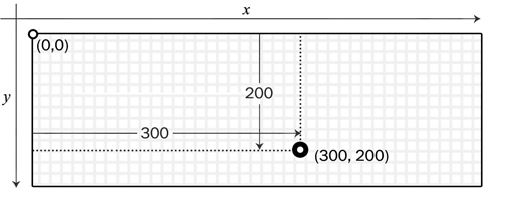
\includegraphics[width=0.5\linewidth]{obrazky/suradnice1}
		\caption{Súradnicový systém plátna s bodom (300, 200) v Snap.svg knižnici}
		\label{fig:suradnice1}
	\end{figure}
\end{center}

\subsection{DOM element}
Sú situácie, kde je potrebné použiť existujúci DOM element ako kontajner pre plátno než viewport. Ako element môžeme použiť napríklad:
\begin{lstlisting}
<div id="mojePlatno"></div>  
\end{lstlisting}

Nasledujúcim kódom vytvorím 500px široké a 300px vysoké plátno.

\begin{lstlisting}
var paper = Snap("mojePlatno", 500, 300);
\end{lstlisting}

Keď využívam túto formu konštruktora, tak prvý element je ID elementu. Alternatívne sa dá prvý parameter DOM element napísať nasledovným spôsobom: 
\begin{lstlisting}
Snap(document.getElementById('mojePlatno'), 500, 300);
\end{lstlisting}



\subsubsection{\acs*{SVG} v HTML dokumente}

SVG môže byť zobrazená buď ako inline v HTML dokumente, alebo ako vloženým samostatného .SVG súboru. 
V tabuľke \ref{vytvorenie:SVG} sú vymenované HTML tagy na zobrazenie SVG. 


\begin{table}[H]
	\begin{center}
		\begin{tabular}{|l|l|}
			\hline \textbf{Technika (tag)} & \textbf{Popis} \\ 
		
			\hline $<$embed$>$ & Načíta vytvorený SVG súbor.  \\ 
			\hline $<$object$>$ & Vytvorí objekt SVG  \\ 
			\hline $<$iframe$>$ & Zobrazí SVG v rámci  \\ 
			\hline Inline $<$svg$>$ & Vytvorí SVG   \\ 
			\hline 
		\end{tabular} 
	\end{center}
	\caption{Spôsoby vytvorenia SVG v HTML dokumente}
	\label{vytvorenie:SVG}
\end{table}

%%%%%%%%%%%%%%%%%%%%%%%%%%%%%%%%%%%%%%%%%%%%%%%%%%%%%%%%%%%%%%%%%%%%%%%%%%%%%%%%%%%%%%%%%%%%%%%%%%%%%%%%%%%%%%%%%%%%%%%%%%%%%%%%%%%%%%%%%%%%%%%%%%%%%%%%%%%%%%%%%%%%%%%%%%%%%%%%%%%%%%%%%%%%%%%%%%%%%%%%%%%%%%%%%%%%%%%%%


\section{Kreslenie základných tvarov cez knižnicu Snap.svg}

Snap API poskytuje metódy na kreslenie jednoduchých tvarov uvedené v tabuľke \ref{porovnanieSVG:Snap}.

\begin{table}[H]
	\begin{center}
		\begin{tabular}{|l|l|l|l|}
			\hline \textbf{Tvar} & \textbf{SVG element} & \textbf{Snap API} & \textbf{Atribúty} \\ 
			\hline
			\hline Obdlžnik & $<$rect$>$ & .rect() & x, y, šírka, výška, rx, ry \\ 
			\hline Kruh & $<$circle$>$ & .circle() & r, x, y, cx, cy, rx, ry \\ 
			\hline Elipsa & $<$ellipse $>$ & .ellipse() & x, y, cx, cy, rx, ry \\ 
			\hline Čiara & $<$line$>$ & .line() & x1, y1, x2, y2 \\ 
			\hline Polyline & $<$polyline$>$ & .polyline() & pole x, y súradnic bodov \\ 
			\hline Polygon & $<$polygon$>$ & .polygone() & pole x, y súradnic bodov \\ 
			\hline Path & $<$path$>$ & .path() & vid tabuľka \ref{prikazy:Path}  \\ 
			\hline 
		\end{tabular} 
		
	\end{center}
	
	\label{porovnanieSVG:Snap}
	\caption{Zoznam tvarov, ktoré podporuje SVG a Snap API}
\end{table}




Tvar, ktorý je vykreslený cez Snap API má nasledovnú syntax: 

\begin{lstlisting}
var paper = Snap(...);
var tvar = paper.NazovSnapMetody({
nazovAtributu: "hodnotaAtributu",
...
});
\end{lstlisting}

Tvar, ktorý je vykreslený priamo na HTML webovej stránke má vo vnútri elementu $<$svg$>$ definované atribúty nasledujúcim spôsobom: 

\begin{lstlisting}
<ElementTvar nazovAtributu = "hodnotaAtributu" ... />
\end{lstlisting}


\subsection{Popis atribútov tvarov}

Názvy atribútov a ich význam pre obdĺžnik, kruh, elipsu sú vyjadrené v tabuľke \ref{parametre:tvar} 

\begin{table}[H]
	\begin{center}
		\begin{tabular}{|l|l|}
			\hline \textbf{Parameter} & \textbf{Poznámka} \\ 
			\hline
			\hline x, y & súradnica x-osi, y-osi  \\ 
			
			\hline cx & x-os súradnica centra kruhu, alebo elipsy \\ 
			\hline cy & y-os súradnica centra kruhu, alebo elipsy \\ 
			\hline r & polomer kruhu, elipsy alebo okruhlých rohov na obdĺžniku \\ 
			\hline rx & horizontálny polomer elipsy \\ 
			\hline ry & vertikálny polomer elipsy \\ 
			\hline x1, y1 & začiatočné x, y súradnice \\
			\hline x2, y2 & konečné x, y súradnice \\
			
			%\hline width, height & šírka, výška\\
			\hline
		\end{tabular} 
		
	\end{center}
	\caption{Názvy atribútov a ich význam}
	\label{parametre:tvar}
\end{table}

Pre útvary polyline, polygon sú atribúty dvojice súradníc osi x, y, ktoré určujú body, ktoré sa spoja. 



\subsubsection{Path tvar}


V Snap API je to metóda Paper.path([pathString]), ktorá vytvorí $<$path$>$ element podľa daného reťazca.  Parameter pathString pozostáva reťazca skladajúceho sa z jedno písmenkových príkazov, nasledovanými bodkami a oddeľovaný argumentami a číslami. Príkazy sú uvedené v tabuľke \ref{prikazy:Path}.

Napríklad: "M10,20L30,40" - obsahuje príkazy: M s argumentami (10, 20) a L (30, 40). Rozdiel vo veľkosti písma v príkaze vyjadruje to, či ide o absolútnu, alebo relatívnu cestu. Ak sú malé znaky jedná sa o relatívne, v prípade veľkých znakov absolútna cesta. 


\begin{center}
	\begin{table}[H]
		\begin{center}
			\begin{tabular}{|c|l|c|}
				\hline \textbf{Príkaz} & \textbf{Názov} & \textbf{Parametre} \\
				\hline
				\hline M & moveto & (x y)+ \\ 
				\hline Z & closepath & (none) \\ 
				\hline L & lineto & (x y)+ \\ 
				\hline H & horizonal lineto & x+ \\ 
				\hline V & vertical lineto & y+ \\ 
				\hline C & curveto & (x1 y1 x2 y2 x y)+ \\ 
				\hline S & smooth curveto & (x2 y2 x y)+ \\ 
				\hline Q & quadratic Bézier curveto & (x1 y1 x y)+ \\ 
				\hline T & smooth quadratic Bézier curveto & (x y)+ \\ 
				\hline 
			\end{tabular} 
		\end{center}
		\caption{Príkazy na tvorbu Path elementu}
		\label{prikazy:Path}
	\end{table}
\end{center}


\section{Vykreslenie obrázku}
Snap povoľuje vloženie bitmapových obrázkov (.jpg alebo .png) na plátno. Používa metódu image z Paper objektu. Parametre metódy image sú: zdroj, x, y, šírka, výška. Príklad kódu, ktorý vkladá .jpg obrázok do plátna:
\begin{lstlisting}
var paper = Snap("mojePlatno", 300, 200);
paper.image("obrazok.jpg", 15, 15, 100, 150);
\end{lstlisting}


\section{Atribúty elementu}

Tvary, ktoré sa dajú nakresliť sa môžu vyfarbiť, orámovať alebo mnoho iných atribútov sa dá nastaviť. Keď sa vytvorí tvar, tak sa vráti Element objekt. Tento objekt má attr metódu, ktorá akceptuje key-value pár atribútov. V tomto odseku sa pozrieme na rôzne atribúty, ktoré môžu byť aplikované na naše grafické komponenty používajúc túto metódu. 

%Element.attr(...) vráti alebo nastaví dané atribúty elementu. Medzi parametre patrí buď objekt, ktorý sa skladá s páru kľúč-hodnota, alebo názvu atribútu. 

\subsection{Výplň elementu - fill }

Pozadie pre element nastavím cez metódu attr použitím fill atribútu ako parameter. Pre jednofarebné výplne je formát vyjadrený cez CSS špecifikáciu. CSS špecifikácia farieb je nasledovná: \#rrggbb alebo skrátene \#rgb , rgb(r, g, b) reťazec alebo slovne. 
Napríklad: 
\begin{lstlisting}
var kruh = paper.circle(50, 50, 40).attr("fill", "red");
\end{lstlisting}

Ďalšie spôsoby výplne elementu sú obrázkom,  gradientom, alebo vzorom. 
Pre nastavenie neprehľadnosti nastavíme atribút opacity na hodnotou čísla v rozsahu od 0-1. Element bude neviditeľný pri hodnote opacity: 0. 
 

\subsection{Nastavenie okraja elementu - stroke}

Elementy môžu mať niekoľko rôznych druhov okrajových atribútov. Prehľad tých najznámejších je v tabuľke \ref{parametre:styl}.\cite{styly}


\begin{table}[H]
	\begin{center}
		
		\begin{tabular}{|l|l|l|}
			\hline \textbf{Atribút pre attr() } &\textbf{CSS atribút} & \textbf{Poznámka} \\ 
			\hline 
			
			\hline stroke & stroke & farba výplne okraja \\ 
			\hline strokeWidth & stroke-width & šírka okraja v px, default je 1 \\ 
			\hline
			strokeOpacity & stroke-opacity & neprehľadnosť, 0-1 \\
			\hline strokeLinecap & stroke-linecap & ["butt", "square", "round"], tvar - okraj konca\\ 
			\hline strokeLinejoin & stroke-linejoin & ["bevel", "round", "miter"], tvar - okraj roku\\ 
			
			\hline strokeDasharray &stroke-dasharray & pole čiarok, bodiek.., napr.5,3,2\\
			
			\hline
		\end{tabular} 
	\end{center}
	\caption{Výber možných stroke atribútov}
	\label{parametre:styl}
\end{table}


\section{Zoskupovanie elementov}

Niekedy je potrebné použiť rovnaké atribúty, transformácie, alebo animácie pre viacero elementov. V Snap API je možné využiť metódu group alebo g. Group zoskupí viacero elementov do množiny. Príkazom add sa dajú pridať ďalšie prvky. V množine sa dajú meniť atribúty pre viacero prvkov naraz volaním metódy attr. 

Príklad zoskupenia elementov. Výsledné zoskupenie je zobrazené na obrázku \ref{fig:grupovanieElementov}. 

\begin{lstlisting}
var paper = Snap();
var kruh = paper.circle(50, 50, 40);
var obdlznik = paper.rect(120, 10, 80, 80);
var elipsa = paper.ellipse(270, 50, 40, 20);

var skupina = paper.g(kruh, obdlznik);
skupina.add(elipsa);

skupina.attr({
	fill: 'yellow',
	stroke: '#000',
	strokeWidth: 5, 
	strokeDasharray: [3, 5, 1]
});
\end{lstlisting}

\begin{figure}[H]
\centering
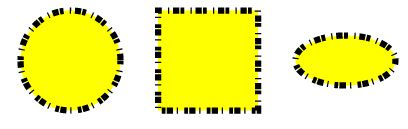
\includegraphics[width=0.7\linewidth]{obrazky/grupovanieElementov}
\caption{Príklad zoskupenia elementov a následná zmena atribútov}
\label{fig:grupovanieElementov}
\end{figure}



\section{Gradient} 

Snap.svg podporuje aplikovanie gradientov cez atribút fill s parametrom stringu gradientu. 



\subsubsection{Linerárny gradient}
Syntax pre lineárny gradient je $<$uhol$>$-$<$farba$>$[-$<$farba$>$[:$<$offset$>$]]*-$<$farba$>$ . Vyjadruje to gradient nakreslený v určitom uhle z prvej do druhej farby.\\ Napríklad rect.attr({fill: '0-\#f00-\#00f'}); . 
Príklad využitia v SCADA systéme je teplomer. 

\subsubsection{Radiálny gradient}
Syntax pre radiálny gradient je r[($<$fx$>$, $<$fy$>$)]$<$farba$>$[-$<$farba$>$[:$<$offset$>$]]*-$<$farba$>$ . 
Vykresľuje radiálne smerom von z fixovaného bodu na elemente. \\Napríklad circle.attr({fill:'r\#fff-000'});




%
%
%\newpage
%\clearpage
%TOTO BUDE PRIKLAD KED BUDEM MAT UZ NAPISANE ATTRIBUTY NA ZMENU STYLU
%asi by bolo velmi vhodne pouzit nejake ine demo, ako ubohy kruh, teda asi teplomer, alebo mapu, ale urcite nieco ine ako kruh!!!!!!!!!!
%
%\subsubsection{PRIKLAD TVORBY KRUHU A NASTAVENIE ATRIBUTOV }
%
%Kód vytvoreného kruhu: 
%
%\begin{lstlisting}
%<svg width="100" height="100">
%<circle cx="50" cy="50" r="40" stroke="black" stroke-width="2" fill="silver" />
%</svg>	
%\end{lstlisting}
%
%SVG obrázok začína s $<$svg$>$ elementom. Atribúty elementu $<$svg$>$ sú width a height. Definujú šírku a výšku SVG obrázka. Element $<$circle$>$ je použitý na nakreslenie kruhu.
%
%
%TODO TODO TODO
%
%Atribúty stroke a stroke-width určujú to ako bude vyzerať obrys útvaru. Kruh má nastavený 2px čierny okraj. 
%Atribút fill vyplní vnútro kruhu. V príklade je vyplnený sivou farbou. Tag, ktorý uzavrie SVG obrázok je $<$$/$svg$>$. Keďže SVG je validné XML, tak všetky elementy musia byť správne zatvorené. \cite{inline}
%
%Kruh vytvorený cez Snap API má nasledovný kód:
%
%\begin{lstlisting}
%var paper = Snap(100, 100);
%var kruh = paper.circle(50, 50, 40);
%kruh.attr({
%stroke: "black", 
%strokeWidth: 2, 
%fill: "silver"
%});
%
%\end{lstlisting}
%
%
%Vykreslí sa na HTML stránku obrázok \ref{jednoduchyKruh}. Obidva spôsoby vykreslili kruh na webovej stránke úplne rovnako.  
%
%\begin{figure}[hp]
%	\begin{center}
%		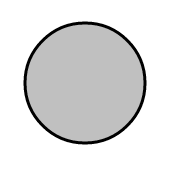
\includegraphics  {obrazky/jednoduchyKruh.png}
%		\caption{Vykreslený kruh vytvorený cez SVG, a Snap API}
%		\label{jednoduchyKruh}
%	\end{center}
%\end{figure}
%
%

%\subsection{Maskovanie - Element.mask()}
%TODO - 
%PRE DANY ELEMENT VOLAM FUNKCIU ATTR, KDE NASTAVIM VLASTNOST MASK 
%NAPR. mask: ellipse
%
%/ Now more interesting stuff
%// Let's assign this group as a mask for our big circle
%bigCircle.attr({
%	mask: discs
%});

\section{Práca s textom - Paper.text(x, y, text)}

Vykreslenie textu na plátne namiesto HTML markup s CSS štýlovaným umožňuje animovať a transformovať v rovnakým spôsobom ako iné tvary. Text vytvorení cez metódu text. Parametre metódy text sú súradnice x, y a text, ktorý sa vykreslí. Vlastnosti textu sa dajú zmeniť volaním metódy attr. V tabuľke sú atribúty, ktoré sa dajú zmeniť prostredníctvom metódy attr. 


\begin{table}[H]
	
	\begin{center}
		
		\begin{tabular}{|l|l|p{8cm}|}
			\hline \textbf{Snap atribút}  &\textbf{ CSS atribút}  & \textbf{Poznámka} \\ 
						\hline
			\hline font & font & napr. "30px Helvetica, sans-serif",\\ 
			\hline textAnchor & text-anchor & pozícia textu, napr. "middle" \\ 
			\hline fill & fill & výplň textu farbou, gradientom, vzorom \\ 
			\hline fontSize  & font-size  & veľkosť textu  \\ 
			\hline fontFamily & font-family & napr. "monospace" \\ 
			\hline fontStyle & font-style  & štýl písma, napr. kurzíva  \\ 
			\hline fontVariant  & font-variant  & napr. "small-caps"  \\ 
			\hline  fontWeight & font-weight  &  hrúbka písma,  napr. normal, bold, bolder, lighter, 100-900\\ 
			\hline 
		
		\end{tabular} 
		
		
	\end{center}
\label{tab:text}
\caption{Atribúty na zmenu vlastností elementu text}
\end{table}

Príklad zmeny farby: 
\begin{lstlisting}
var paper = Snap();
var text = paper.text(30, 100, "Namestovo");

text.attr({
	textAnchor: "middle",
	fill: "#00b", 
	fontSize: '16px', 
	fontFamily: "Veranda", 
	fontStyle: "italic", 
	fontVariant: "small-caps", 
	fontWeight: 800, 
});
\end{lstlisting}

Na obrázku \ref{fig:textPriklad} je zobrazený text, ktorý bol uvedený v príklade. 

\begin{figure}[H]
\centering
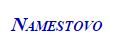
\includegraphics{obrazky/textPriklad}
\caption{Príklad na zmenu atribútov v texte.}
\label{fig:textPriklad}
\end{figure}




\section{Transformácie - Element.transform(...)}


%
%"t100,100r30,100,100s2,2,100,100r45s1.5"
%Each letter is a command. There are four commands: t is for translate, r is for rotate, s is for scale and m is for matrix.
%
%There are also alternative “absolute” translation, rotation and scale: T, R and S. They will not take previous transformation into account. For example, ...T100,0 will always move element 100 px horisontally, while ...t100,0 could move it vertically if there is r90 before. Just compare results of r90t100,0 and r90T100,0.
%
%So, the example line above could be read like “translate by 100, 100; rotate 30 stupnov around 100, 100; scale twice around 100, 100; rotate 45 stupnov around centre; scale 1.5 times relative to centre”. As you can see rotate and scale commands have origin coordinates as optional parameters, the default is the centre point of the element. Matrix accepts six parameters.
%
%Usage
%\begin{lstlisting}
%
%
%var el = paper.rect(10, 20, 300, 200);
%// translate 100, 100, rotate 45, translate -100, 0
%el.transform("t100,100r45t-100,0");
%// if you want you can append or prepend transformations
%el.transform("...t50,50");
%el.transform("s2...");
%// or even wrap
%el.transform("t50,50...t-50-50");
%// to reset transformation call method with empty string
%el.transform("");
%// to get current value call it without parameters
%console.log(el.transform());
%\end{lstlisting}



%
%
%
%Keď vytváram element v Snap, tak efektívne vytváram \ac{DOM} objekt. TODO... \cite [page~51] {Dawber} 
%
%\subsection{Suradnicovy system}

\subsection{Jednoduché transformácie}

Transformácia je realizovaná cez metódu Element.transform(), ktorá má v parametri transformačný string. Pri transformácii sa dá využiť klonovanie elementov cez metódu Element.clone(). Syntax transformačného stringu je vyjadrené z príkazov, ktoré sú v tabuľke \ref{tab:trasf}. 

\begin{table}[H]
	
	\begin{center}
		
		\begin{tabular}{|c|c|c|c|}
			\hline \textbf{Názov} & \textbf{Príkaz} & \textbf{Parameter} & \textbf{Príklad} \\ 
			\hline Posunutie & T, t & x, y & t50,100 \\ 
			\hline Rotácia& R, r & uhol, (bod rotacie x, y) & r45,0,0 \\ 
			\hline Škála & S, s & scale x, y, (scale bod x, y) & S 2,4.5,75,125 \\ 
			\hline 
		\end{tabular} 	
	\end{center}
	\label{tab:trasf}
	\caption{Syntax transformačného stringu pre Snap API}
	
\end{table}

Transformačný string využíva malé a veľké varianty príkazov. Variant s veľkými písmenami znamená to, že sa transformuje, bez ohľadu na predchádzajúcu transformáciu. Opačne to je pri variante s malými písmenami, ktoré berú na vedomie predošlú transformáciu.\cite[p.~52]{Dawber} 

V SVG sa vytvorí k elementu nový tag animateTransform, kde sa nastaví attributeName na transform, a typ a hodnoty sú uvedené v tabuľke \ref{tab:svgTrans}. 

\begin{table}[H]
	\begin{center}
		\begin{tabular}{|l|p{9cm}|}
			\hline \textbf{Transformation} & \textbf{Popis} \\ 
			\hline translate(x,y) & Posunie súradnicový systém na dané x, y.  \\ 
			\hline scale(xFactor, yFactor) & zmena mierky, ak je uvedená len jedna hodnota, prehliadač predpokladá, že obidve hodnoty sú rovnaké. \\ 
			\hline rotate(uhol) & Zrotuje súradnice o daný uhol. Stred rotácie je (0,0).  \\ 
			\hline rotate(uhol, centerX, centerY) & Zrotuje súradnice o daný uhol, s danými súradnicami stredu rotácie.  \\ 
			\hline skewX(uhol) &  Skosenie pozdĺž osi X.  \\ 
			\hline skewY(uhol) &  Skosenie pozdĺž osi Y.  \\ 
			\hline 
		\end{tabular} 
		
	\end{center}
	\label{tab:svgTrans}
	\caption{Typy transformácií vo vnútri SVG tagu animateTransform }
\end{table}
%
%\section{Pracovanie s maticami}
%
%Metóda Snap.matrix(a, b, c, d, e, f) vráti maticu nastavenú podľa daných parametrov.
%Matica je obdĺžníková matica elementov zoradených v riadkoch a stĺpcoch. Konvencia špecifikuje číslo riadka ako prvé, keď sa referuje veľkosti matice. Každý element v matici môže byť považovaný ako komponent, ktorý mapuje niektoré body do ďalšieho budu. ---TODO, ALEBO TO VYHODIM


\section{Animácie}

Snap.svg umožňuje animovať SVG grafické komponenty priamo manipulovaním jeho atribútov v JavaScripte. 

Element.animate(attr, ms, easing, callback). 
Parametre sú v tabuľke \ref{fig:animacie}
\begin{table}[H]
	\begin{center}
		\begin{tabular}{|c|p{10cm}|}
			\hline \textbf{Parameter} & \textbf{Popis} \\ 
			\hline attr &   Atribúty požadovaného elementu sú zadané v pároch - typ atribútu a jeho hodnota \\ 
			\hline duration &   Trvanie animácie v milisekundách \\ 
			\hline easing & zjemnenie animácie, mina objekt \\ 
			\hline callback & Funkcia, ktorá sa spustí po skončení animácie  \\ 
			\hline 
		\end{tabular} 
	\end{center}

	\caption{Parametre pre metódu animate}
		\label{fig:animacie}
\end{table}

\subsubsection{Animácia metód a jednoduchých atribútov animácie }

Jednoduché atribúty elementov, ktorých prechod sa zanimuje sú v časti o atribútoch elementov. Ako atribút sa dá použiť aj CSS3 atribút, ale musí byť v úvodzovkách, ak neexistuje v knižnici Snap.svg jeho ekvivalentný názov. 

\subsubsection{Animovanie path}

Pre animovanie zmeny tvaru jedného grafického komponentu na druhý sa využíva atribút path. Grafický element sa plynulo zanimuje, pretvaruje na tvar, ktorý je udaný. 

\subsection{Animácie transformácie}

Animovanie transformácie atribútu elementu využíva transformačný string.  Syntax: 
\begin{lstlisting}
	Element.animate({transform: [transformacny string]});
\end{lstlisting}




\section{Ďalšie metódy v knižnici Snap.svg}

\subsection{Snap.load(url, callback, [scope])}
Načíta externý .svg súbor ako fragment. 


\subsection{Element.append(...), Element.add(...), }
Slúži na pridanie, zobrazenie elementu na danom plátne. 

\subsection{Snap.select(...)}
Slúži na wrapovanie DOM elementu špecifikovaný CSS selektorom. 






%\begin{table}[H]
%	
%	\begin{center}
%		\begin{tabular}{|p{3cm}|p{3cm}|p{3cm}|p{3cm}|}
%			\hline \textbf{Animacia} & \textbf{SVG akcia} & \textbf{JavaScript akcia} & \textbf{Popis} \\ 
%			\hline Animácia &  &  &  \\ 
%			\hline Nastavenie farby &  &  &  \\ 
%			\hline Transformácia &  &  &  \\ 
%			\hline Skryvanie  &  & attr({visibility: true}) &  \\ 
%			\hline Atributy farby & animateColor  & attr({fill: farba}) &  \\ 
%			\hline  &  &  &  \\ 
%			\hline Nastavenie atributov & set element & metoda attr &  \\ 
%			\hline zmena farby & animateColor element & attr(fill: farba) &  \\ 
%			\hline animovanie transformacie & animateTransform element & transform() &  \\ 
%			\hline  & animateMotion element &  &  zoznam atributov pridate este\\ 
%			\hline  &  &  &  \\ 
%			\hline  &  &  &  \\ 
%			\hline 
%			
%			\hline 
%		\end{tabular} 
%	\end{center}
%	
%	\caption{Mapovacia tabuľka}
%	\label{haha2}
%\end{table}




%V SVG SMIL animacia používa na animáciu elementy, :
%V tabuľke \ref{haha2} je
%
%\begin{table}[H]
%\begin{center}
%	
%\begin{tabular}{|c|c|c|}
%	\hline Názov & Elementy v SVG SMIL & Metódy v Snap.svg.js \\ 
%	\hline Animácia & animate & Element.animate(...) \\ 
%	\hline Nastavovanie & set & Element.attr(...) \\ 
%	\hline Animovanie pohybu & animateMotion & Element.animate(..) \\ 
%	\hline Transformácia & animateTransform & Element.animate({transform: ..}) \\ 
%	\hline 
%\end{tabular} 	\caption{Animovanie v SVG SMIL a v Snap.svg.js }
%	\label{haha2}
%\end{center}
%\end{table}
%
%
%O čom bude táto časť: 
%\begin{itemize}
%	\item Animácia metód a jednoduchých atribútov animácie TODO ZMENA FARBY INDIKATORA 
%	\item Animovanie path TODO KAPITOLA O NADRZI
%	\item Easing využívajúc kubickú Bézierovú syntax
%	\item Animácie transformácie TODO KAPITOLA ROTOR
%	\item Animácie využívajúce spoločné atribúty a animácie popri path TODO MAPA CESTY
%\end{itemize}
%
%\section{Animacia - Element.animate(...)}
%Snap.animation = function (attr, ms, easing, callback) 
%\begin{itemize}
%	\item	- attr (object) atribúty finalného produktu
%	\item	- duration (number) trvanie animácie v milisekundách , 
%	\item - easing (function) vid tabluka, alebo kapitola o tom 	funkcie  @mina 
%	\item funkcia, ktorá sa vykoná po skončení animácii
%\end{itemize}
%
%
%
%\subsection{Animácia atribútov}
%TODO NAPR ZMENA FARBY INDIKATORA TOKU VODY
%
%tabulka ake atributy sa daju menit
%napr
%\begin{itemize}
%	\item visibility: / attr({visibility: true})
%	\item okrajov: pozri tabulku c. \ref{parametre:styl}
%	\item farby: pozri tabulku 
%	\item textu: tabulka \ref{tab:text}
%	\item tvarov: tabulka \ref{parametre:tvar}
%\end{itemize}
%
%
%
%\subsection{Animácia elementov, path}
%TODO NAPR ANIMOVANIE ZMENY PRITOKU VODY DO NADRZE
%%\subsection{Animation easing}
%%Easing describes how the value of an attribute varies with regard to time. By default,
%%the value of an attribute changes consistently—that is, linearly—over the course of
%%an animation but by specifying a particular easing type, we can change the way in
%%which the attribute is animated. Consider the following graph that demonstrates
%%three of the available easing types\ref{fig:easing}:
%%\cite{Dawber}[p~70]
%%
%%\begin{figure}[H]
%%	\centering
%%	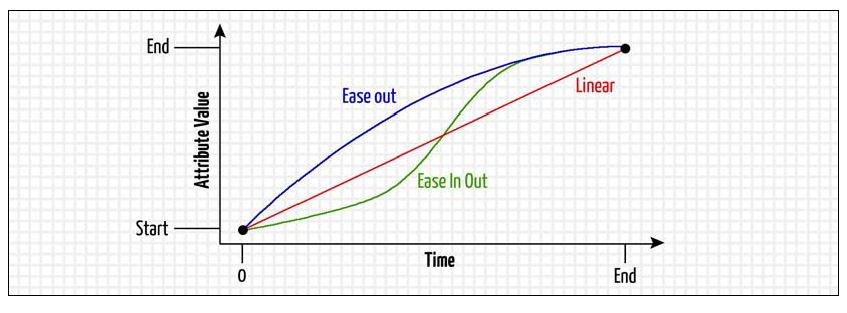
\includegraphics[width=0.7\linewidth]{obrazky/easing}
%%	\caption{Graf troch easing typov}
%%	\label{fig:easing}
%%\end{figure}
%%
%%
%%For each easing type, the rate at which the attribute changes varies along the graph in
%%the time axis. Each easing type can be described as such:
%%\begin{itemize}
%%	
%%	
%%	\item Linear: The value varies consistently from its start value to its end value over
%%	the course of the animation
%%	\item Ease Out: The value increases quickly towards its end point before slowing
%%	down towards the end of the animation
%%	\item Ease In Out: The value decreases slowly at first and then increases quickly
%%	before finally slowing down to its end point towards the end of the animation
%%\end{itemize}
%%
%%
%%
%
%\subsection{Animácia transformácií}
%TODO ASI TEN VENTIL BY BOLO VHODNE ZANIMOVAT A TRANSFORMOVAT
%
%\subsection{Animacia vyuzivajuca vlastne atributy}
%
%\subsection{Animacia podla path}
%toto uz v prikladoch mam ako mapu TODO /
%todo urobit pri nadrzi 
%
%
%
